\documentclass[aspectratio=169]{beamer}

\useoutertheme{infolines}

\usepackage{graphicx}
\usepackage{subcaption}

\title{PNLSS Identification}
\subtitle{Post Institute Meeting 2}
\author[Balaji, N. N.]{Nidish Narayanaa Balaji}
\institute[Rice U.]{Rice University, Houston, TX 77005}
\date{September 26, 2019}
\begin{document}
\maketitle{}

\begin{frame}
  \frametitle{PNLSS for Benchmark 5 (unilateral spring)}
  \begin{itemize}
  \item A HCB reduced model was used for the transient simulations for
    computational tractability
  \end{itemize}
\end{frame}

\begin{frame}
  \frametitle{PNLSS for Benchmark 5 (unilateral spring)}
  \framesubtitle{Number of states: 2; Nonlinearity order: [2, 3]}
  \begin{figure}
    \centering
    \begin{subfigure}{0.25\linewidth}
      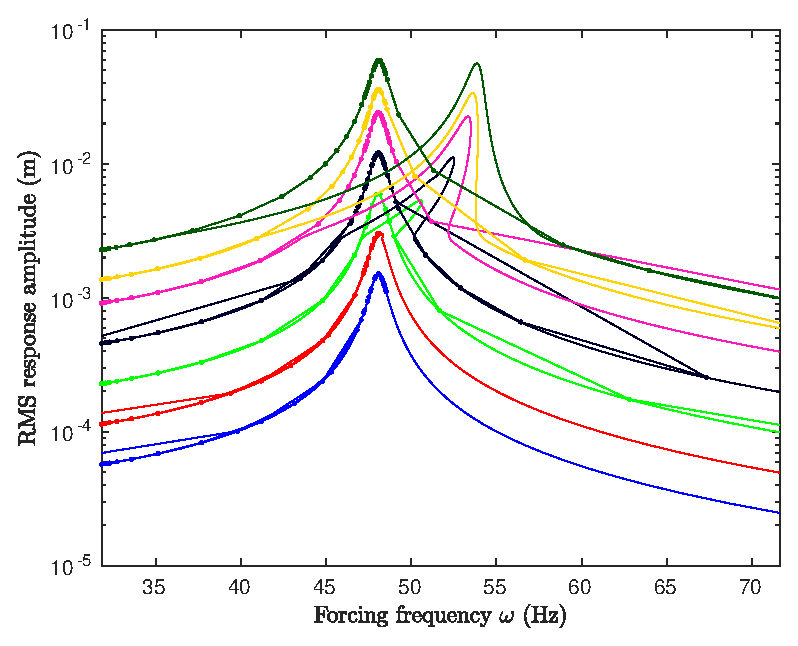
\includegraphics[width=\linewidth]{../../benchmark5/FIGURES/pnlssfrf_Amp_b5_A15_up4_ms_full_na2_nx23}
      \caption{A=15 N}
    \end{subfigure}%
    \begin{subfigure}{0.25\linewidth}
      \includegraphics[width=\linewidth]{../../benchmark5/FIGURES/pnlssfrf_Amp_b5_A30_up4_ms_full_na2_nx23}
      \caption{A=30 N}
    \end{subfigure}%
    \begin{subfigure}{0.25\linewidth}
      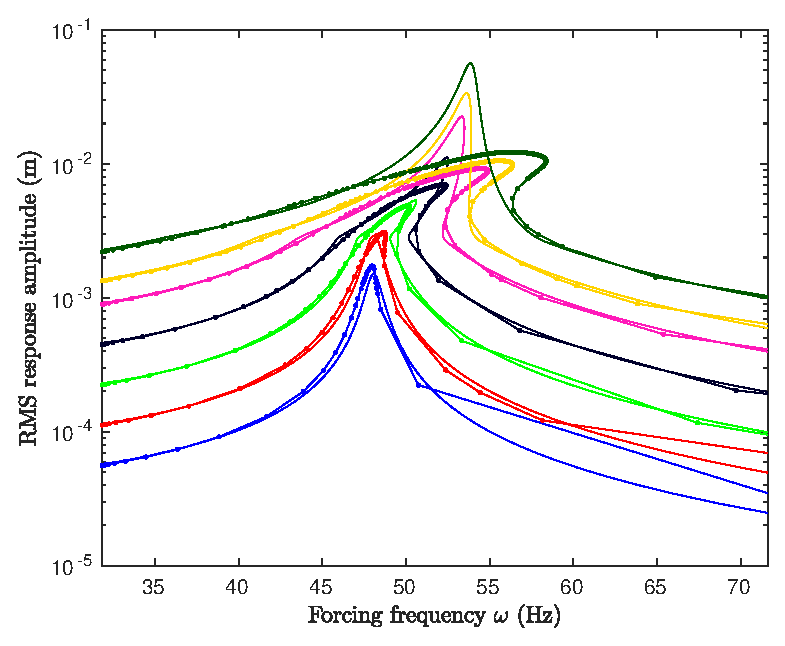
\includegraphics[width=\linewidth]{../../benchmark5/FIGURES/pnlssfrf_Amp_b5_A60_up4_ms_full_na2_nx23}
      \caption{A=60 N}
    \end{subfigure}%
    \begin{subfigure}{0.25\linewidth}
      \includegraphics[width=\linewidth]{../../benchmark5/FIGURES/pnlssfrf_Amp_b5_A120_up4_ms_full_na2_nx23}
      \caption{A=120 N}
    \end{subfigure}
  \end{figure}
\end{frame}

\begin{frame}
  \frametitle{PNLSS for Benchmark 5 (unilateral spring)}
  \framesubtitle{Number of states: 3; Nonlinearity order: [2, 3]}  
  \begin{figure}
    \centering
    \begin{subfigure}{0.25\linewidth}
      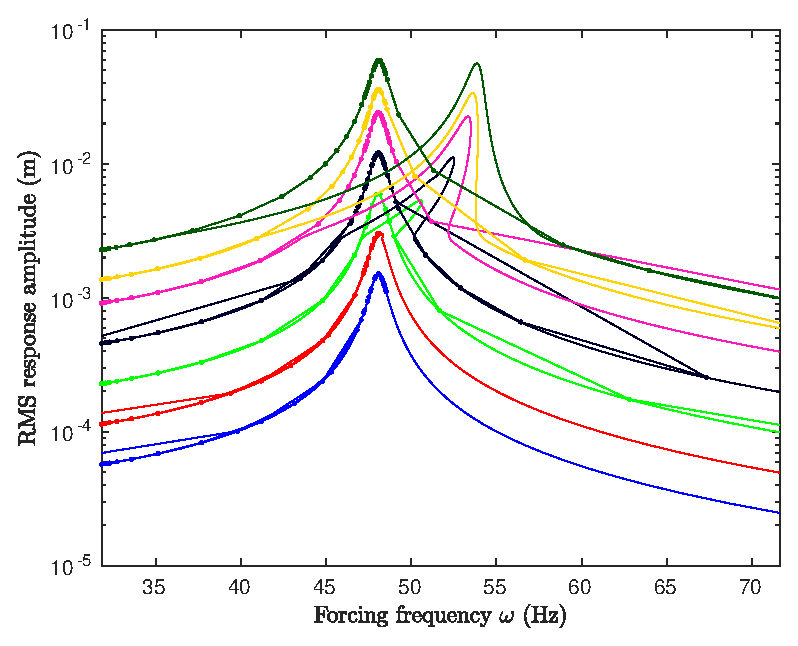
\includegraphics[width=\linewidth]{../../benchmark5/FIGURES/pnlssfrf_Amp_b5_A15_up4_ms_full_na2_nx23}
      \caption{A=15 N}
    \end{subfigure}%
    \begin{subfigure}{0.25\linewidth}
      \includegraphics[width=\linewidth]{../../benchmark5/FIGURES/pnlssfrf_Amp_b5_A30_up4_ms_full_na2_nx23}
      \caption{A=30 N}
    \end{subfigure}%
    \begin{subfigure}{0.25\linewidth}
      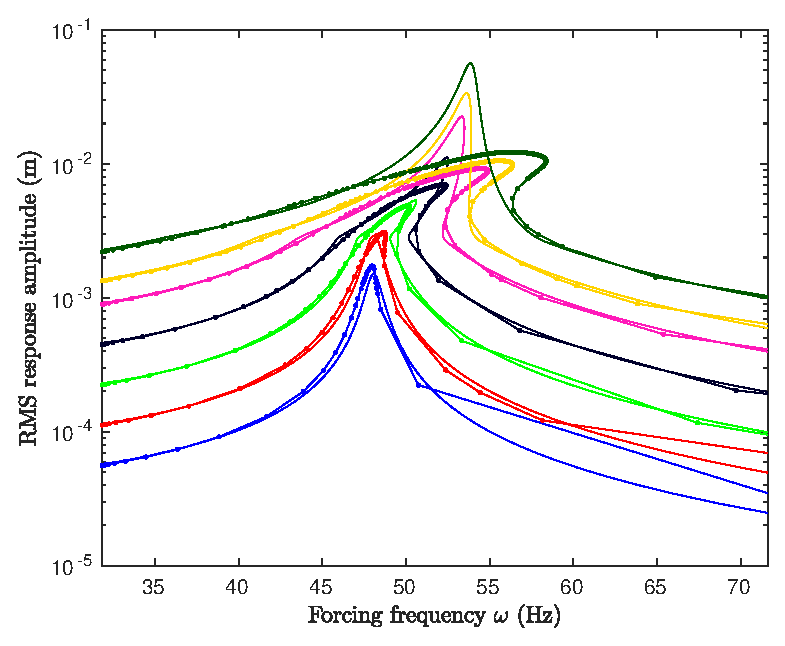
\includegraphics[width=\linewidth]{../../benchmark5/FIGURES/pnlssfrf_Amp_b5_A60_up4_ms_full_na2_nx23}
      \caption{A=60 N}
    \end{subfigure}%
    \begin{subfigure}{0.25\linewidth}
      \includegraphics[width=\linewidth]{../../benchmark5/FIGURES/pnlssfrf_Amp_b5_A120_up4_ms_full_na2_nx23}
      \caption{A=120 N}
    \end{subfigure}
  \end{figure}
\end{frame}

\end{document}
%%% Local Variables:
%%% mode: latex
%%% TeX-master: t
%%% End:
